\documentclass[twocolumn]{article}
\usepackage{tutorial}
%\usepackage{a4}

\oddsidemargin  0.15 in     
\marginparwidth 1 in        %   Width of marginal notes.
%   Note that \oddsidemargin = \evensidemargin
\oddsidemargin  0in    %   Left margin on odd-numbered pages.
\evensidemargin 0in    %   Left margin on even-numbered pages.
\marginparwidth 0.75in
\textwidth 157mm       % Width of text line.
% 1in top margin and 1in bottom margin
\headsep0cm
\headheight0cm
\topmargin-17.4mm
\textheight247mm % A4
\parindent 8pt
\parskip0pt

\usepackage[OT1]{fontenc}

% ------------------------------------------------------------------------
\usepackage{graphicx}
\usepackage{subfigure}
\usepackage{epsfig}
\usepackage{psfrag}
% used to write c++ code/algorithms
\usepackage{listings}
\usepackage{fancyvrb}
\usepackage{path}

%\psdraft

\twocolumn


% hyperref stuff
\usepackage{hyperref}
\hypersetup{
  pdftitle={A Tutorial on CGAL Polyhedron for Subdivision Algorithms},
  pdfauthor={INRIA Geometrica},
  pdfsubject={A tutorial for CGAL},
  pdfkeywords={},
  pdfpagemode=UseThumbs,
  baseurl={http://www.cgal.org},
  colorlinks=true,
  linkcolor=black,
  anchorcolor=black,
  citecolor=black,
  filecolor=black,
  menucolor=black,
  pagecolor=black,
  urlcolor=blue,
  bookmarksopen=false,}
% end hyperref stuff

\lstset{language=C++, basicstyle=\scriptsize}

\graphicspath{{figs/}}
\def\figurename{Figure}
\def\tablename{Tableau}
\newcommand{\italic}[1]{\emph{#1}} 

% ------------------------------------------------------------------------
\newcommand\IL{{\itshape left}}
\newcommand\IR{{\itshape right}}
\newcommand\IM{{\itshape middle}}
\newcommand\IT{{\itshape top}}
\newcommand\IB{{\itshape bottom}}

% ------------------------------------------------------------------------
\newcommand{\CodeFmt}[1]{{\small\texttt{#1}}}

\def\kernel{\CodeFmt{Kernel}}

\def\cgalpoly{\CodeFmt{CGAL::Polyhedron\_3}}
\def\poly{\CodeFmt{Polyhedron\_3}}
\def\polytrait{\CodeFmt{PolyhedronTraits\_3}}
\def\polyitem{\CodeFmt{PolyhedronItems\_3}}
\def\polybuilder{\CodeFmt{Polyhedron\_incremental\_builder\_3}}

\def\cgalhds{\CodeFmt{CGAL::HalfedgeDS}}
\def\hds{\CodeFmt{HalfedgeDS}}
\def\hdsitem{\CodeFmt{PolyhedronItems}}

% L.K. -------------------------------------------------------------------
\newcommand{\CC}{C\raise.08ex\hbox{\texttt{++}}}
\newcommand{\openmesh}{\textsc{OpenMesh}}
\newcommand{\opensg}{\textsc{OpenSG}}
\newcommand{\cgal}{\textsc{Cgal}}
\newcommand{\stl}{\textsc{Stl}}


% =========================================================================
\begin{document}

% TITLE
% ------------------------------------------------------------------------
\date{}
\title{{\LARGE {\sffamily\bfseries A Tutorial on CGAL Polyhedron \\
for Subdivision Algorithms\thanks{%
    Partially supported by the grant NSF 9457806-CCR and
    IST Programme of the EU as a Shared-cost
    RTD (FET Open) Project under Contract No IST-2000-26473 (ECG -
    Effective Computational Geometry for Curves and Surfaces). 
}}}}


\author{\small
\sffamily Le-Jeng Shiue\footnote{SurfLab, University of Florida}
\and \small
\sffamily Pierre Alliez\footnote{GEOMETRICA, INRIA Sophia-Antipolis}
\and \small
\sffamily Radu Ursu\footnote{Geometry Factory, Sophia-Antipolis}
\and \small
\sffamily Lutz Kettner\footnote{Max-Planck-Institut f\"ur Informatik,
    Saarbr\"ucken, Germany}}
\maketitle

\thispagestyle{empty}

\begin{abstract}
  We give an overview of the tutorial for the \texttt{CGAL:: Polyhedron\_3}
  and its use in subdivision algorithms. The full tutorial and the
  accompanying source code are available at
  \path|http://www.cgal.org/Tutorials/Polyhedron/|.
\end{abstract}


% ------------------------------------------------------------------------
\section*{Introduction}

Polyhedron data structures based on the concept of halfedges have been
very successful for the design of general algorithms on meshes.
Common practice is to develop such data structure from scratch, since
clearly a first implementation is at the level of a students homework
assignment. But then, these data structures consist almost entirely of
pointers for all sort of incidence informations. Maintaining them
consistently during mesh operations is not anymore a trivial
linked-list update operation. So, moving from a students exercise to a
reliable research implementation, including maintaining and optimizing
it, is a respectable software task.

What is common practice for simple data structures, such as linked
lists, should be common practice even more so for mesh data
structures, namely, to use a good, flexible, and efficient library
implementation. In \CC\, the \emph{Standard Template Library}, \stl,
is an excellent address for our analog example of the linked
lists~\cite{Austern:1999:GPS}, and we argue in the full tutorial that
the Polyhedron data structure in \cgal\ is such a flexible mesh data
structure~\cite{k-ugpdd-99}, and it comes with a rich and versatile
infrastructure for mesh algorithms. \cgal, the 
\emph{Computational Geometry Algorithms Library}, is a 
\CC\ library available from \path|www.cgal.org|~\cite{fgkss-dccga-00}. 

\begin{figure}[h]
  \centering
  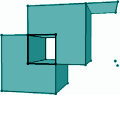
\includegraphics[width=\linewidth]{figs/teaser}
  \caption{The polyhedron viewer running on Windows. A coarse polygon 
    mesh is subdivided using the quad-triangle subdivision scheme.}
  \label{fig:viewer}
\end{figure}

We strongly believe that such a tutorial with its wealth of
information will give a head start to new researches and implementations
of mesh algorithms. We also believe that it will raise the quality of
implementations. Firstly, it encourages the use of well tested and
over time matured implementations, e.g., \cgalpoly\ in its current
design is about five years publicly released and used. Secondly, it
documents good implementation choices, e.g., the example programs can
be used as starting points for evolutionary software development.
Thirdly, it offers easy access to additional functionality, such as
the efficient self intersection test, that otherwise could be
expandable in a research prototype.

The tutorial is organized around subdivision surfaces in a 
polyhedron viewer. The polyhedron viewer
(\figurename\ \ref{fig:viewer}) demonstrates the basic functionalities of
the \cgalpoly\ and some extended functionalities such as file I/O,
mesh superimposition, and trackball manipulation. Several subdivision
surfaces are supported in the polyhedron viewer, including
Catmull-Clark, Loop, Doo-Sabin, $\sqrt{3}$ and Quad-Triangle
subdivisions.  The tutorial shows how to implement subdivision
surfaces in two different mechanisms provided by \cgalpoly :
\emph{Euler operators} and \emph{modifier callback mechanism}.  A
$\sqrt{3}$ subdivision implementation is designed based on the Euler
operators and a Quad-Triangle subdivision implementation is designed
based on overloading the modifier.  Extended from the previous design,
a \emph{combinatorial subdivision library} (CSL) is then proposed with
increased sophistication and abstraction. CSL abstracts the geometry
operations from the refinements. Subdivisions in CSL are build from
refinement host with a template geometry policy. Several fundamental
refinement schemes are provided within CSL. They are instantiated with a
geometry policy that can be user defined.

The goal of this tutorial is to show how to use \cgalpoly\ 
on basic graphics functionalities, such as rendering and 
interactive trackball manipulation, \emph{and} how to design and 
implement algorithms around meshes. Since connectivity and 
geometry operations are the primal implementation components
in mesh algorithms, subdivisions are chosen to
demonstrate both operations on \cgalpoly . 
Hence, readers intended to design and implement 
mesh algorithms other than subdivisions will also be 
benefited from the tutorial.

% ------------------------------------------------------------------------
\subsection*{Intended Audience}

The intended audience of the tutorial are researchers, developers or
students developing algorithms around polyhedron meshes. Knowledge of 
the halfedge data structure and subdivisions are prerequisites. 
Short introductions of these two topics are given in the tutorial.
The tutorial assumes familiarity with the \CC\ template mechanism 
and the key concepts of generic programming~\cite{Austern:1999:GPS}. 


% ------------------------------------------------------------------------
\subsection*{CGAL Polyhedron}

CGAL Polyhedron (\cgalpoly) is realized as a container class 
that manages geometry items such as vertices, halfedges, and 
facets with their incidences.  \cgalpoly\ has chosen the 
halfedge data structure as the underlying connectivity 
structure. In the halfedge data structure, a halfedge is 
associated with a facet and stores the adjacency pointers 
to it previous, next and opposite halfedge (\figurename\ \ref{fig:halfedge}). 
The details of the halfedge data structure and the \cgalpoly\ based 
on it are described in~\cite{k-ugpdd-99}.

\begin{figure}[h]
    \centering{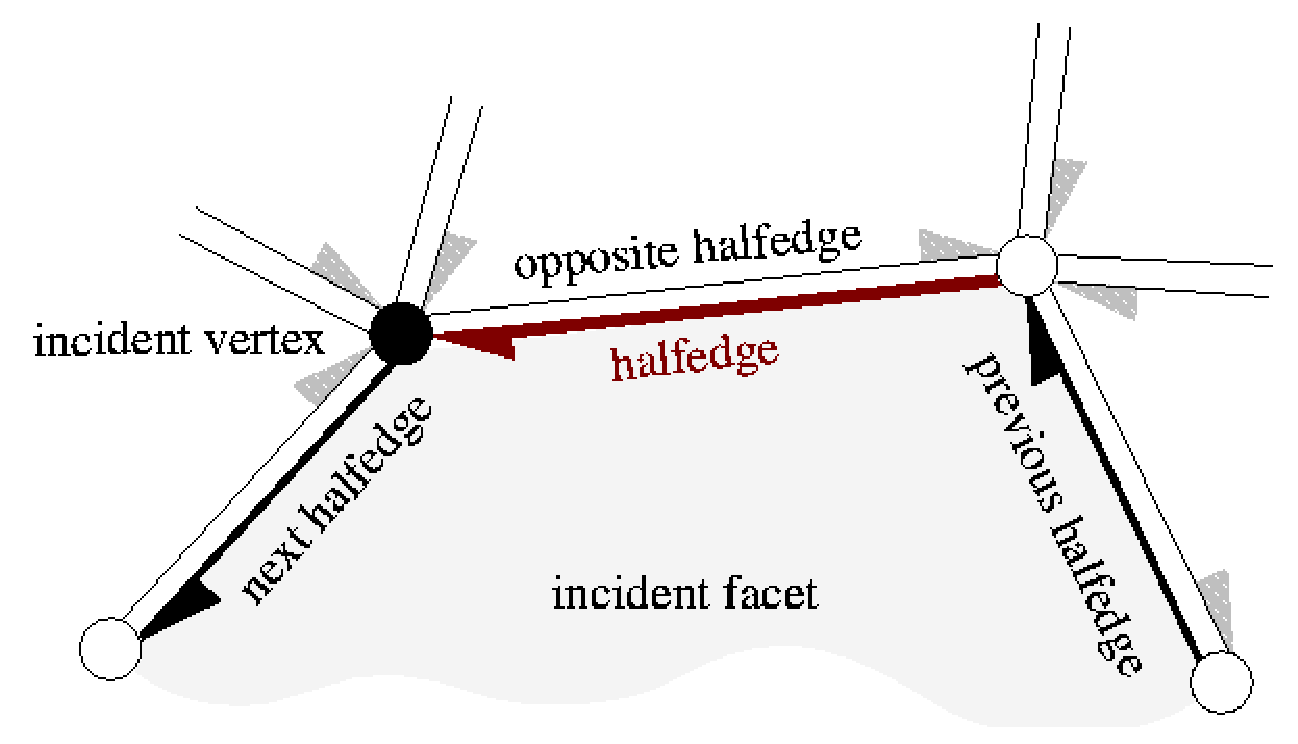
\includegraphics[width=5.0cm]{figs/halfedge}}
    \caption{One halfedge and its incident primitives. The next
      halfedge, the opposite halfedge, and the incident vertex are
      mandatory, the remaining elements are optional.
    }
    \label{fig:halfedge}
\end{figure}

What are the potential obstacles in using CGAL and \cgalpoly?
\begin{enumerate}
  \item
    Is it fast enough? Yes. \cgal, coming from the field of Computational
    Geometry, might have a reputation of using slow exact arithmetic
    to be on the safe side, but nonetheless, we know where to apply
    the right techniques of exact arithmetic to gain robustness and
    yet not to loose efficiency. In addition, \cgal\ uses
    \emph{generic programming\/} and \emph{compile-time
    polymorphism\/} to realize flexibility without affecting optimal
    runtime.
  \item
    Is it small enough? Yes. \CodeFmt{CGAL::Polyhedron \_3} can be
    tailored to store exactly the required incidences and other
    required data, not more and not less.
  \item
    Is it flexible enough? Yes, certainly within its design
    space of oriented 2-manifold meshes with boundary that was
    sufficient for the range of applications illustrated with our
    example programs. 
  \item
    Is it easy enough to use? Yes. The full tutorial with its example
    programs are exactly the starting point for using \cgalpoly. The
    example programs are short and easy to understand. There is
    certainly a learning curve for mastering \CC\ to the level
    of using templates, but it has to be emphasized that
    using templates is far easier then developing templated code.
  \item
    What is the license, can I use it? Yes, we hope so. \cgal\ since
    release 3.0 and our tutorial programs have open source
    licenses. Other options are available.
\end{enumerate}

% ------------------------------------------------------------------------
\subsection*{Subdivision Surfaces}

A subdivision algorithm recursively 
applies \emph{refinement} and \emph{geometry smoothing} 
on the control mesh (\figurename\ \ref{fig:sqrt3},  
\ref{fig:quad-triangle}), 
and approximates the limit surface of the control mesh.  Several
refinement schemes in practice are illustrated in
\figurename\ \ref{fig:RefSchemes}. The stencils of the
geometry smoothing are depending on the refinement schemes, 
i.e.\ the reparameterizations. A stencil defines a control
submesh that is associated with normalized weights of the 
nodes. \figurename\ \ref{fig:RefMap} 
demonstrates the stencils of the PQQ scheme  
in Catmull-Clark subdivision \cite{cc} and DQQ scheme in Doo-Sabin
subdivision \cite{ds}. We also demonstrate Loop \cite{loop}, 
$\sqrt{3}$ \cite{sqrt3} and Quad-Triangle \cite{qts} subdivisions 
in this tutorial. For further details about subdivisions, readers
should refer to \cite{Warren:subdivision} and \cite{Sub:course:2000}.
   
\begin{figure}[tb]
  \centering
  \psfrag{PQQ}[]{\scriptsize PQQ} 
  \psfrag{PTQ}[]{\scriptsize PTQ}
  \psfrag{DQQ}[]{\scriptsize DQQ} 
  \psfrag{Sqrt3}[]{\scriptsize $\sqrt{3}$} 
  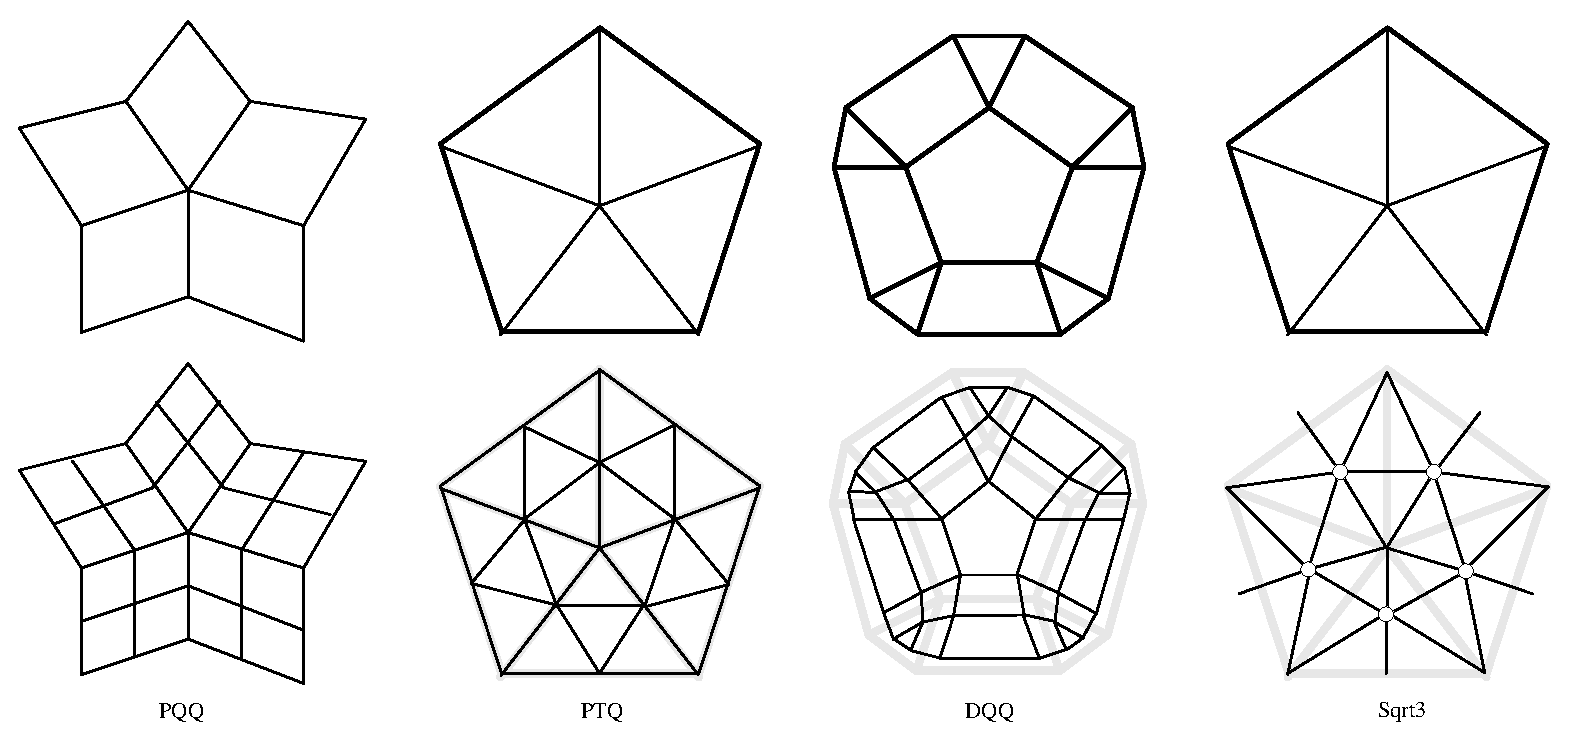
\epsfig{file=figs/RefSchemes.eps, width=7.5cm}
  \caption{Examples of refinement schemes: 
    primal quadrilateral quadrisection (PQQ),
    primal triangle quadrisection (PTQ),
    dual quadrilateral quadrisection (DQQ) and
    $\sqrt{3}$ triangulation. The control meshes are shown
    in the first row.}
  \label{fig:RefSchemes}
\end{figure}

% ------------------------------------------------------------------------
%\section*{(Our) FAQs}

%We compile a list of questions concerned about the tutorial and the
%accompanying source codes and libraray.   
 

%\begin{itemize}

%% \item Why should I read this tutorial? I am not interested in subdivisions. 
%% The goal of this tutorial is to show how to use \cgalpoly\ 
%% on basic graphics functionalities, such as rendering and 
%% interactive trackball manipulation, \emph{and} how to design and 
%% implement algorithms around meshes. Subdivisions are choosen for their
%% connectivity and geometry operations. These two operations are the  
%% primal components in most mesh algorithms. For reader not interested 
%% in subdivisions, the know-how of the connectivity and geometry
%% manipulations is the foundation of mesh algorithm implementations  
%% based on \cgalpoly . 

%% \item Why do you use \cgal\ polyhedron? How about OpenMesh and its 
%% subdivision library?
%% \cgal\ is highly generic and well-tested robust. \cgal\ 
%% and versatile for its geometry 
%% functionalities. The OpenMesh subdivision
%% library is not as generic.

%\item Is is difficult or what's the difficulties to use \cgal\ Polyhedron?
% It is not, once you buy the concepts taken or inspired from
% the STL (iterators, circulars). You also have to be familiar 
% with the concept of handles and halfedges.

%\item How about the performance?
% as fast as other libraries (and sometimes faster). It also
% scales well. 

%\item I don't like the subdivisions you have, how can I build my own 
%      subdivision on your solution?
% depending on the level of genericity you are targeting, the
% type of scheme and whether you want to store all levels of subdivision
% in memory, choose either Euler operators, incremental builder
% or one new template rule to be plugged into the CSL.

%\item What's the future plan for CSL? 
% CGAL Package?
% referenced from Warren's web site about subdivision?

%\item The viewer is based on OpenGL. Can I learn from it
%      to write my own viewer based on another graphics library?
      
%\item What could be improved in the Polyhedron?
% built-in functions for # of boundaries, # of connected 
% components and genus.
% edge collapses without the currently too restrictive precondition
% (along with a function bool is_collapsible(Halfedge_handle h)
% based on e.g. Edelsbrunner criteria.
% built-in function bool is_border(Vertex_handle v)
% built-in function to know the type of mesh (e.g. pure tri,
% pure quad, tri-quad or polygonal).

%\end{itemize}

% ------------------------------------------------------------------------
\section*{Tutorial Outlines}

% ------------------------------------------------------------------------
\subsection*{Polyhedron Viewer}

%% We have designed and implemented an application based on the
%% \cgalpoly. This program provides a polyhedron viewer of
%% following functionalities:\\
%% \indent $\bullet$ File I/O,\\
%% \indent $\bullet$ polyhedron rendering,\\ 
%% \indent $\bullet$ and trackball manipulation.\\
%% In addition to these built-in functions, the viewer is accompanied
%% with a set of subdivision algorithms that generate smooth polyhedron
%% surfaces from a coarse polyhedron. \italic{The tutorial instructs the
%% readers through the design and the implementation of the polyhedron
%% viewer and the subdivisions}. The first part of the tutorial
%% highlights the design and implementation issues related to the \poly\
%% used in the viewer. The second part of the tutorial explains how to
%% implement the connectivity and geometry operations of the subdivision
%% algorithms. The source codes are going to be published with the
%% releasing of the tutorial.

The tutorial starts with an implementation of 
a basic polyhedron viewer based on the \cgalpoly\ with the 
default configuration.
This basic viewer demonstrates basic functionalities of a 
\cgalpoly . We describe how to import a polyhedron file in 
the OFF format based on the \italic{modifier callback mechanism} and the 
\italic{incremental builder}. We also show the mesh traversal based on
the \italic{iterators} and the \italic{circulators} for rendering and 
the OFF file exporting. 

An extended polyhedron viewer is then introduced by customizing 
the \poly\ with extra attributes and functionalities. This 
enriched polyhedron supports facet and vertex normals for rendering, 
supports the axis-aligned bounding box of the polyhedron, and 
provides geometry items specialized with algorithmic flags. 
%The extended primitives are employed to support efficient 
%computation of the number of connected components, number 
%of boundaries and combinatorial genus of the polyhedron. 
The superimposition of the control mesh on the subdivision surfaces
are implemented with the flags of the halfedge items 
(\figurename\ \ref{fig:quad-triangle}). 
%This enriched polyhedron is used as
%the core data structure of our application. 

The tutorial also features a trackball to interactively manipulate the
polyhedron, a snapshot function of the camera viewpoint and 
the transformation states, a raster output to the clipboard, and the
vectorial output to a postscript file.% (\figure\ \ref{fig:gargoyle}).

\begin{figure}[h]
  \centering
  \psfrag{A}[]{(a)}
  \psfrag{B}[]{(b)}
  \psfrag{C}[]{(c)}
  \psfrag{D}[]{(d)}
  \epsfig{file=figs/RefMap.eps, width=7.5cm}
  \caption{The stencil ({\itshape top blue}) and its 
           vertex ({\itshape bottom red}) in 
           Catmull-Clark subdivision (a-c)
           and Doo-Sabin subdivision (d). Catmull-Clark
           subdivision has three stencils: facet-stencil (a), 
           edge-stencil (b) and vertex-stencil (c). 
           Doo-Sabin subdivision has only corner-stencil (d).
           The stencil weights are not shown.}
  \label{fig:RefMap}
\end{figure}

%% \begin{figure}[t]
%%     \centering{\includegraphics[width=3.5cm]{figs/gargoyle_raster}
%%                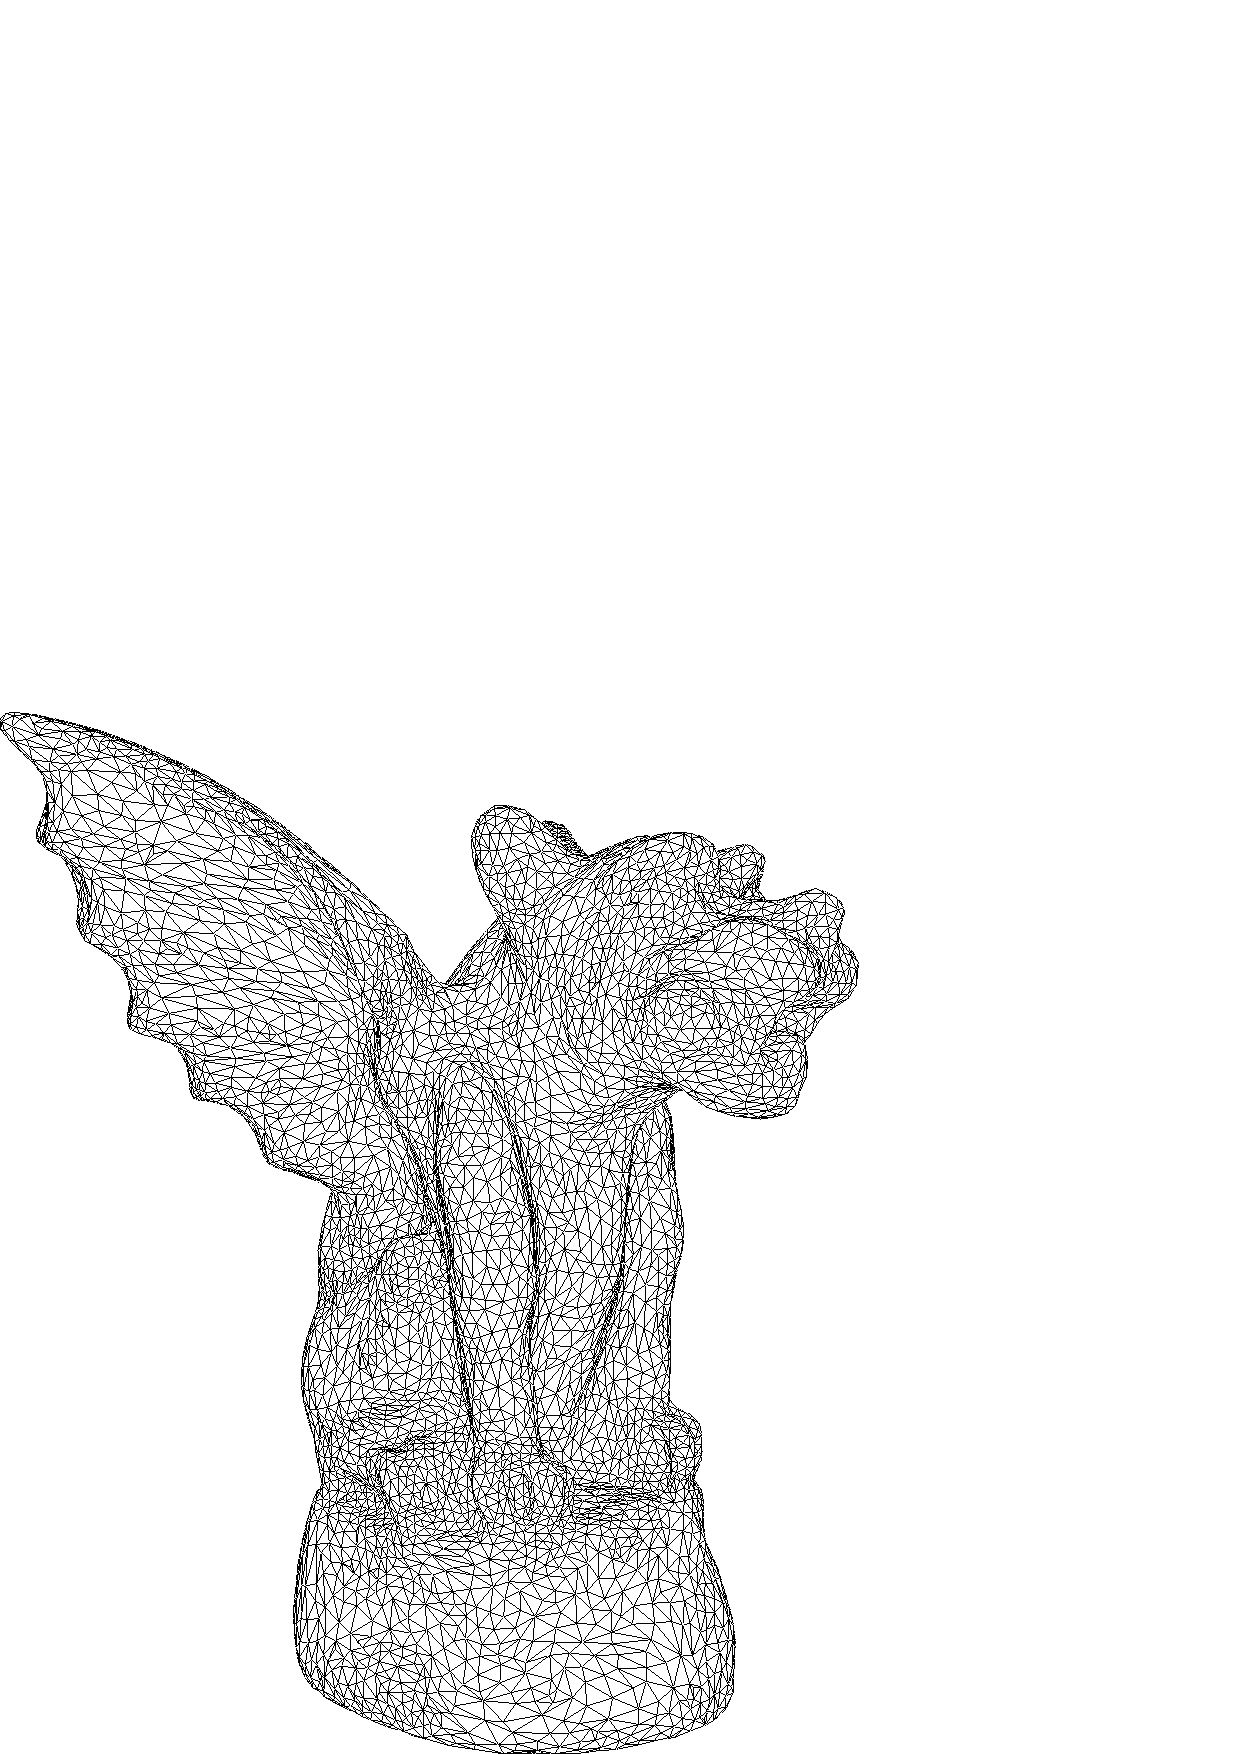
\includegraphics[width=3.5cm]{figs/gargoyle_vec}}
%%     \caption{Raster and vectorial output of the gargoyle mesh.}
%%     \label{fig:gargoyle}
%% \end{figure}

% ------------------------------------------------------------------------
\subsection*{Subdivision Algorithms}

The second part of the tutorial focuses on the design and the
implementation of $\sqrt{3}$ subdivision (\figurename\ \ref{fig:sqrt3}) 
and Quad-Triangle subdivision (\figurename\ \ref{fig:quad-triangle}).  

In addition to its importance in the surface modeling, we 
choose subdivision algorithms to demonstrate both the 
\italic{connectivity operation} (refinement) and the
\italic{geometry operation} (smoothing) of a
\cgalpoly . These two operations are the
primary implementation components required by algorithms on
polyhedron meshes. Readers intended to design and implement
mesh algorithms other than subdivisions will also be benefited
from the techniques we proposed here.

The key to implement a subdivision algorithm is to 
efficiently support the refinement, i.e.\ the connectivity 
modifications. Two approaches are introduced to support the 
refinement: the \italic{Euler operators} (operator scheme) and
the \italic{modifier callback mechanism} (modifier scheme). 
The operator scheme reconfigures the connectivity with a 
combination of Euler operators. $\sqrt{3}$ subdivision~\cite{sqrt3} is
used to demonstrate this scheme. We also compare our implementation
with the $\sqrt{3}$ subdivision provided in OpenMesh library.

Though simple and efficient in some
refinements, e.g.\ $\sqrt{3}$ subdivision, the correct combination of
the operators is hard to find for some refinements, e.g.\ Doo-Sabin
subdivision~\cite{ds}. The modifier scheme solves the problem by
letting the programmers create their own combinatorial operators 
using the polyhedron incremental builder. Quad-Triangle
subdivision~\cite{qts,l-pg-03} is used to demonstrate this scheme.

% ------------------------------------------------------------------------
\subsection*{Combinatorial Subdivision Library}

The \emph{C}ombinatorial \emph{S}ubdivision \emph{L}ibrary 
(CSL) is designed based on the policy-based design 
\cite{Alexandrescu:2001:MCD}.
The policy-based design assembles a class
(called \emph{host}) with complex behavior out of many 
small behaviors (called \emph{policies}).
Each policy defines an interface for a
specific behavior. CSL proposes a 
generic subdivision solution as a \emph{refinement function}
parameterized with the \emph{geometry smoothing rules}.
Subdivisions in CSL are build as proper combinations of the
refinement functions and the geometry policy classes.
The refinement function refines the control mesh,
maintains the correspondence between the control mesh and refined
mesh, and applies the smoothing stencils provided by the policy
class. For example, Catmull-Clark subdivision~\cite{cc} is structured
\begin{figure}[h]
    \centering{\includegraphics[width=7.0cm]{figs/sqrt3}}
    \caption{$\sqrt{3}$ subdivision of the mannequin mesh.}
    \label{fig:sqrt3}
    \vspace{0.5cm}
\end{figure}
as a quadralization function parameterized with the Catmull-Clark
smoothing rules.


\begin{lstlisting}
void CatmullClark_subdivision(Polyhedron& p) {    
  quadralize_polyhedron
                <CatmullClark_rule<Polyhedron>>(p);  
}
class CatmullClark_rule {
public:
  void facet_rule(  Facet_handle  facet, Point& pt);
  void edge_rule(Halfedge_handle   edge, Point& pt);
  void vertex_rule(Vertex_handle vertex, Point& pt);
};
\end{lstlisting}
\noindent The \CodeFmt{quadralize\_polyhedron<>()} 
is the host function refining the input mesh
and the \CodeFmt{CatmullClark\_rule} is the policy 
class applying the Catmull-Clark stencils.
The refinement functions are implemented based on the
Euler operations or the modifier callback mechanism.
The refinement functions also maintain the 
correspondence with the stencil, i.e., the submesh 
centered around the given facet, edge, or
vertex, and the smoothing point.
The smoothing point is calculated by calling the 
policies, e.g., the \CodeFmt{facet\_rule()}, the 
\CodeFmt{edge\_rule()}, and the \CodeFmt{vertex\_rule()} 
respectively. Inside a policy, applying the 
stencil is simplified to the mesh traversal of a 
1-ring neighborhood which can be done with the 
circulators. Following example illustrates  
the policy of the facet-stencil in Catmull-Clark 
subdivision.
\begin{lstlisting}
void facet_rule(Facet_handle facet, Point& point) {
  Halfedge_around_facet_circulator hcir 
                            = facet->facet_begin();
  Vector vec = hcir->vertex()->point() - ORIGIN;
  ++hcir;
  do {
    vec = vec + hcir->vertex()->point();
  } while (++hcir != facet->facet_begin());
  point = ORIGIN + vec/circulator_size(hcir);
}
\end{lstlisting}

\begin{figure}[h]
    \centering{\includegraphics[width=7.5cm]{figs/quad-triangle}}
    \caption{Quad-Triangle subdivision of the rhombicuboctahedron mesh.}
    \label{fig:quad-triangle}
\end{figure}

This policy-based approach offers a convenient way to
specialize a subdivision with the template smoothing rules.
CSL currently supports Catmull-Clark, 
Loop, Doo-Sabin, $\sqrt{3}$ and Quad-Triangle
subdivisions. %(\figurename\ \ref{fig:subzoo}).
Though demonstrated with a specific enriched \poly\ in our 
polyhedron viewer, CSL accepts any polyhedron mesh specialized 
from the \poly\ with the \CodeFmt{Point} type defined in the vertex.  
%not just the enriched polyhedron we used in the polyhedron
%viewer.

%% \begin{figure}[tb]
%%   \centering
%% %  \epsfig{file=figs/rook.eps, width=2cm}
%%   \epsfig{file=figs/rook_cc.eps, width=1.3cm}
%%   \epsfig{file=figs/rook_ds.eps, width=1.3cm}
%%   \epsfig{file=figs/rook_qt.eps, width=1.3cm}
%%   \epsfig{file=figs/rook_loop.eps, width=1.3cm}
%%   \epsfig{file=figs/rook_sqrt3.eps, width=1.3cm}
%%   \caption{Subdivisions supported in CSL.}
%%   \label{fig:subzoo}
%% \end{figure}


% references
{\footnotesize
\bibliographystyle{alpha}
\bibliography{abstract}
}

\end{document}
